\documentclass{report}

%====================== PACKAGES ======================
\usepackage{listings}
\usepackage{xcolor}

\definecolor{codegreen}{rgb}{0,0.6,0}
\definecolor{codegray}{rgb}{0.5,0.5,0.5}
\definecolor{codepurple}{rgb}{0.58,0,0.82}
\definecolor{backcolour}{rgb}{0.95,0.95,0.92}

\lstdefinestyle{mystyle}{
    backgroundcolor=\color{backcolour},
    commentstyle=\color{codegreen},
    keywordstyle=\color{magenta},
    numberstyle=\tiny\color{codegray},
    stringstyle=\color{codepurple},
    basicstyle=\ttfamily\footnotesize, 
    breaklines=true,
    numbers=left,
    numbersep=5pt,
    captionpos=b,
    frame=single
}
\lstset{style=mystyle, language=Java}

\usepackage[english]{babel}
\usepackage[utf8]{inputenc}
\usepackage[T1]{fontenc}
\usepackage{float}
\usepackage{amsmath}
\usepackage{amssymb}
\usepackage{graphicx}
\usepackage{array}
\usepackage{tabularx}
\usepackage{booktabs}
\usepackage{enumitem}
\usepackage{setspace}
\usepackage{abstract}
\usepackage{subfig}
\usepackage{pdflscape}
\usepackage{textcomp}
\usepackage{eurosym}
\usepackage[top=2cm, bottom=2cm, left=2cm, right=2cm]{geometry}
\usepackage[hidelinks]{hyperref}

% Allow the literal euro sign in the source text.
\DeclareUnicodeCharacter{20AC}{\euro{}}

% Look for images in this folder and in the shared UML folder.
\graphicspath{{./}{../uml/}}

%====================== SETTINGS ======================
\setcounter{secnumdepth}{3}
\setcounter{tocdepth}{2}

\newcommand{\HRule}{\rule{\linewidth}{0.5mm}}
\newcommand{\code}[1]{\texttt{#1}}
\newcolumntype{Y}{>{\raggedright\arraybackslash}X}

%======================== DOCUMENT ========================
\begin{document}

% Cover page
\begin{titlepage}
\begin{center}

% Logo

\includegraphics[width=0.6\textwidth]{./logo}\\[1.5cm]

% Institution
\textsc{\LARGE CentraleSupélec}\\[0.5cm]
\textsc{\Large 2EL1520 -- Génie logiciel orienté objet}\\[1.5cm]

% Title
\HRule \\[0.5cm]

{\huge \bfseries Supermarket Checkout System\\[0.3cm]}
{\Large \bfseries Object-Oriented Software Engineering Project\\[0.5cm]}

\HRule \\[1.5cm]

% Group info
\textbf{\large Author:}\\[0.5cm]

Enzo Jardim Vendramin\\

\vspace{2cm}

% Additional info
\textbf{Teacher:} Paolo Ballarini\\[0.3cm]
\textbf{Academic Year:} 2025--2026\\[2cm]

\vfill

% Date
{\large 31 May 2026}

\end{center}
\end{titlepage}

\thispagestyle{empty}

\tableofcontents
\thispagestyle{empty}
\newpage

%====================== CONTENT ======================
\chapter{Introduction}
\label{ch:introduction}

\textit{[Skeleton --- to be written.]}

\section{Context and Objectives}
\textit{Brief presentation of the assignment: a supermarket checkout system in
Java with a command-line interface, graded on design quality, design patterns,
JUnit tests and UML. State the goals of this report.}

\section{Scope and Deliverables}
\textit{What is delivered: the Java implementation, the test scenarios, this
report and the UML diagrams; pointer to the GitHub repository.}

\section{Report Structure}
\textit{One sentence describing the remaining chapters.}


\part{The Specified System}
\label{part:specified}
% Everything required by the project instructions (R1--R10, the CLUI and the
% mandatory tests) is developed in this part.
\chapter{Requirements and Design Decisions}
\label{ch:requirements}

This chapter recalls the functional requirements, shows that each of them is
implemented and tested, and explains the main design decisions they induced.

\section{Functional Requirements}
The core requirements (R1--R10) describe a checkout that treats purchases as a
set of bought items in mandatory categories (R1, R2, R2b), where each item is
priced and the price may depend on the quantity (R3), and payment is made by
bank card (R4). The system must offer \emph{extensible} discount plans --- at
least \emph{prime} (20\% off when the total reaches \euro{}50) and \emph{platinum}
(30\% off always) --- and let the owner introduce new ones (R5, R5b). It must
apply \emph{category-level pricing policies} that are likewise extensible (R6,
R6b). Customers may request home delivery (R7), charged according to weight and
distance, with refusal above 50\,kg (R8) and plan-based reductions (R8b).
Finally, the system maintains a live inventory that raises low-stock alerts
using the Observer pattern (R9) and supports two-hour delivery slots with
anti-overbooking and dynamic pricing (R10). Part~2 of the assignment adds a
command-line user interface (CLUI) and mandatory tests.

\section{Requirements Traceability}
\label{sec:traceability}
Table~\ref{tab:traceability} shows that every element required by the
instructions is implemented and tested. It maps each requirement to the classes
that realise it and to the JUnit tests (or scenario) that validate it.

\begin{table}[H]
\centering
\small
\begin{tabularx}{\linewidth}{p{1.6cm} Y Y}
\toprule
\textbf{Req.} & \textbf{Implemented in} & \textbf{Validated by} \\
\midrule
R1, R2, R2b & \code{Cart}, \code{CartEntry}, \code{Item}, \code{Category}; \code{Supermarket.setup} & \code{CliDispatcherTest}, \code{BillComputationTest} \\
R3 & \code{Item.unitPriceFor} (quantity-based price) & \code{ItemTest} \\
R4 & \code{POSDevice}, \code{TransactionAuthorisationSystem}, \code{BankCard} & \code{PaymentFlowTest}, \code{TransactionAuthorisationSystemTest} \\
R5 & \code{DiscountPlan} + Normal/Prime/Platinum & \code{DiscountPlanTest}, \code{BillComputationTest} \\
R5b & \code{DiscountPlanFactory}, \code{getAnnualFee} & \code{DiscountPlanTest}, \code{SupermarketTest} \\
R6, R6b & \code{PricingPolicy}, \code{CategoryDiscount} & \code{PricingPolicyTest} \\
R7 & \code{DeliveryRequest}, \code{Supermarket.requestDelivery} & \code{DeliveryCheckoutTest} \\
R8 & \code{StandardDeliveryCalculator} & \code{DeliveryCalculatorTest} \\
R8b & \code{DiscountPlan.applyDeliveryDiscount} & \code{DiscountPlanTest}, \code{DeliveryCheckoutTest} \\
R9 & \code{Inventory}, \code{StockObserver} (Observer) & \code{InventoryObserverTest} \\
R10 & \code{TimeSlot}, \code{DeliveryManager} & \code{DeliveryManagerTest}, \code{TimeSlotTest} \\
Customer ID (\S2.3) & \code{Customer.numericalId} & \code{SupermarketTest} \\
CLUI (Part 2) & \code{cli} package (login, setup, scanItem, pay, runTest, \ldots) & \code{CliDispatcherTest} \\
Test scenario (\S4) & \code{testScenario1.txt}, \code{my\_supermarket.ini} & \code{CliDispatcherTest} \\
\bottomrule
\end{tabularx}
\caption{Requirements traceability: every required feature is implemented and tested.}
\label{tab:traceability}
\end{table}

\section{How Requirements Shaped the Design}
Two words in the instructions drove most of the design: \emph{extensible} and
\emph{Observer}. The requirement to add new discount plans (R5b) and new pricing
policies (R6b) without modifying existing code led directly to the
\textbf{Strategy} pattern: discount plans and pricing policies are interfaces
with interchangeable implementations, so a new plan or policy is a new class
rather than an edit to the checkout. The same reasoning applies to the delivery
charging scheme (R8). The explicit demand for the \textbf{Observer} pattern in
R9 shaped the inventory module, where the stock count is decoupled from whoever
reacts to a shortage.

Three further decisions are worth noting. First, the bank-side protocol (R4) is
hidden behind a single \emph{authorise} operation, a \textbf{Facade} that keeps
the rest of the system independent of the banking details. Second, the code is
organised in layers (domain entities, services, orchestration, user interface)
so that the business logic does not depend on the way it is driven --- a property
that proved valuable when a second interface was later added. Third, all
monetary output is produced with a fixed locale (period decimals, UTF-8), so the
computed figures are identical on any machine that grades the project.

\section{The Bill Computation Pipeline}
\code{CashRegister.computeBill()} is the heart of the specified system. For the
items in the cart it applies, in order:
\begin{enumerate}[nosep]
  \item the \textbf{quantity-based unit price} (R3), through
  \code{Item.unitPriceFor(qty)};
  \item the \textbf{category pricing policy} (R6), e.g.\ a 10\% reduction on
  fruit and vegetables;
  \item the customer's \textbf{discount plan} (R5) on the resulting subtotal ---
  prime applies its 20\% only when that subtotal reaches \euro{}50, platinum
  always applies 30\%;
  \item the \textbf{delivery fee} (R8) when a delivery was requested, reduced by
  the plan (R8b: prime pays half, platinum free).
\end{enumerate}
The total is thus \emph{items after plan} plus \emph{plan-adjusted delivery}.
Subscribing to a plan also charges its annual fee immediately (normal
\euro{}0, prime \euro{}50, platinum \euro{}200), as required by \S2.3.

\chapter{Architecture and Design Patterns}
\label{ch:architecture}

\textit{[Skeleton --- to be written.]}

\section{Package Architecture}
\textit{Layered overview of the packages (model, services, register, cli, gui)
and the dependency direction.}

\section{Design Patterns}
\textit{Describe each pattern and the problem it solves.}

\begin{table}[H]
\centering
\begin{tabularx}{\linewidth}{p{2.2cm} Y}
\toprule
\textbf{Pattern} & \textbf{Where and why} \\
\midrule
Strategy & \textit{Discount plans, pricing policies, delivery, promotions (placeholder).} \\
Observer & \textit{Inventory low-stock alerts (placeholder).} \\
Factory & \textit{Discount-plan creation by name (placeholder).} \\
Facade & \textit{Transaction Authorisation System (placeholder).} \\
Command & \textit{Undo/redo of scans (placeholder).} \\
\bottomrule
\end{tabularx}
\caption{Design patterns used (to be completed).}
\label{tab:patterns}
\end{table}

\section{Domain Core and Orchestration}
\textit{Role of \code{Supermarket} (system core) and \code{CashRegister}
(checkout orchestration).}

\chapter{UML Diagrams}
\label{ch:uml}

This chapter presents the UML models of the specified system. Because the full
class diagram is large, it is shown here as focused per-package views (each
legible on its own); the complete class diagram is provided in
Appendix~\ref{app:fullclass}. The extension classes are shown separately in
Part~\ref{part:extensions}.

\section{Class Diagram (per package)}
\label{sec:class-diagram}
\textit{[Commentary to be written.]}

\begin{figure}[H]
    \centering
    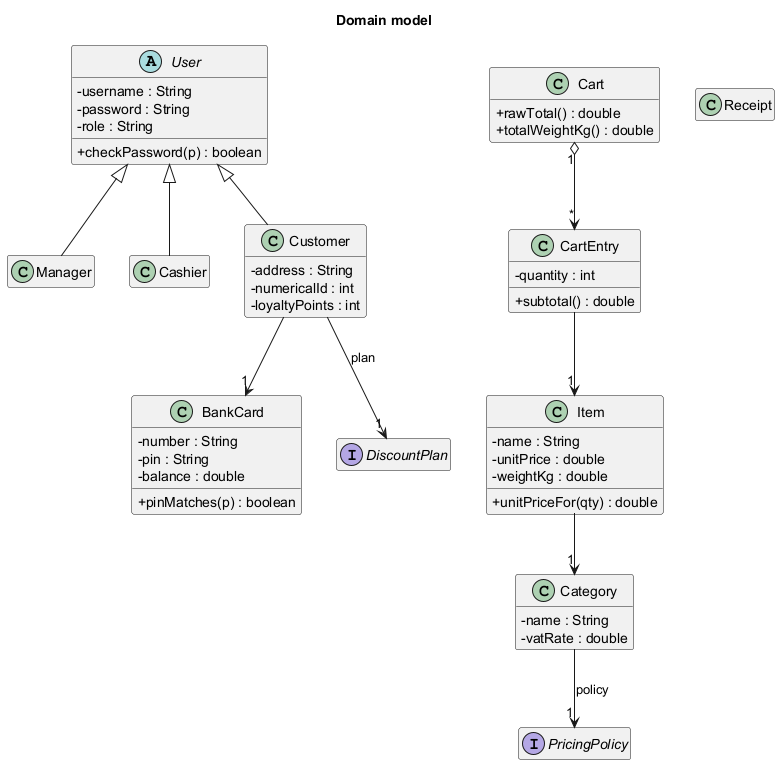
\includegraphics[width=0.95\linewidth]{class-domain.png}
    \caption{Domain model: entities, the user hierarchy and their relationships.}
    \label{fig:class-domain}
\end{figure}

\begin{figure}[H]
    \centering
    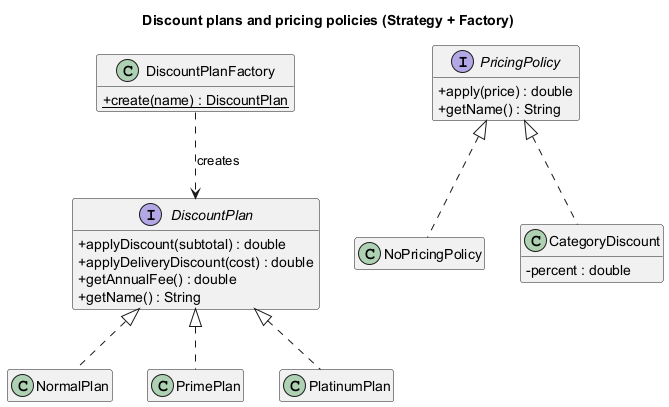
\includegraphics[width=0.95\linewidth]{class-discount-pricing.png}
    \caption{Discount plans and pricing policies (Strategy + Factory).}
    \label{fig:class-discount}
\end{figure}

\begin{figure}[H]
    \centering
    \subfloat[Inventory and alerts (Observer).]{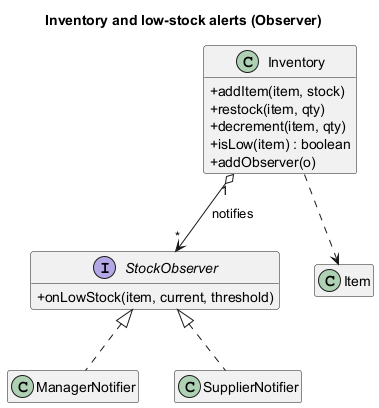
\includegraphics[width=0.46\linewidth]{class-inventory.png}}
    \hfill
    \subfloat[Payment (Facade).]{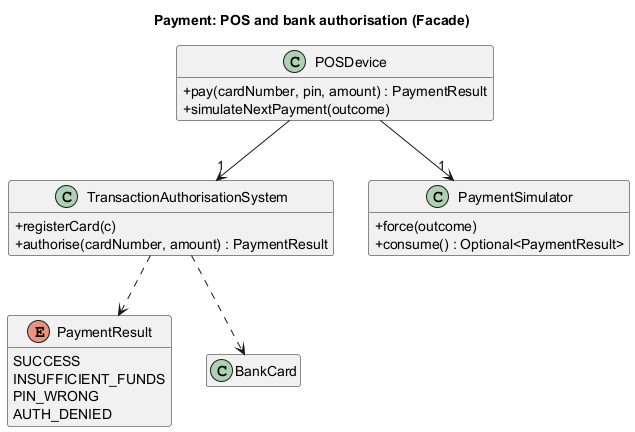
\includegraphics[width=0.46\linewidth]{class-payment.png}}
    \caption{Inventory/Observer (left) and Payment/Facade (right).}
    \label{fig:class-inv-pay}
\end{figure}

\begin{figure}[H]
    \centering
    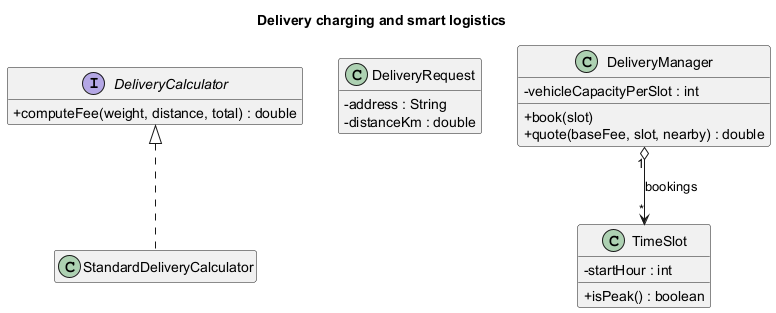
\includegraphics[width=0.8\linewidth]{class-delivery.png}
    \caption{Delivery charging (Strategy) and smart-logistics classes.}
    \label{fig:class-delivery}
\end{figure}

\begin{figure}[H]
    \centering
    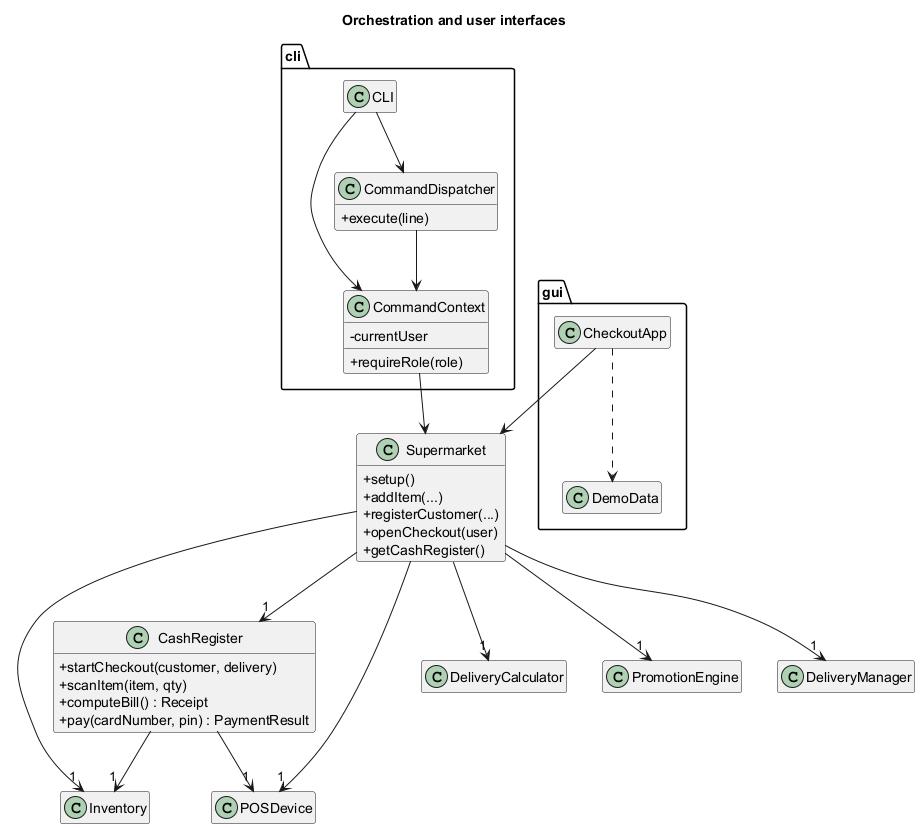
\includegraphics[width=0.85\linewidth]{class-orchestration.png}
    \caption{Orchestration core (\code{Supermarket}, \code{CashRegister}) and the
    two user interfaces.}
    \label{fig:class-orchestration}
\end{figure}

\section{Use-Case Diagram}
\label{sec:use-case}
\textit{[Commentary to be written.]}

\begin{figure}[H]
    \centering
    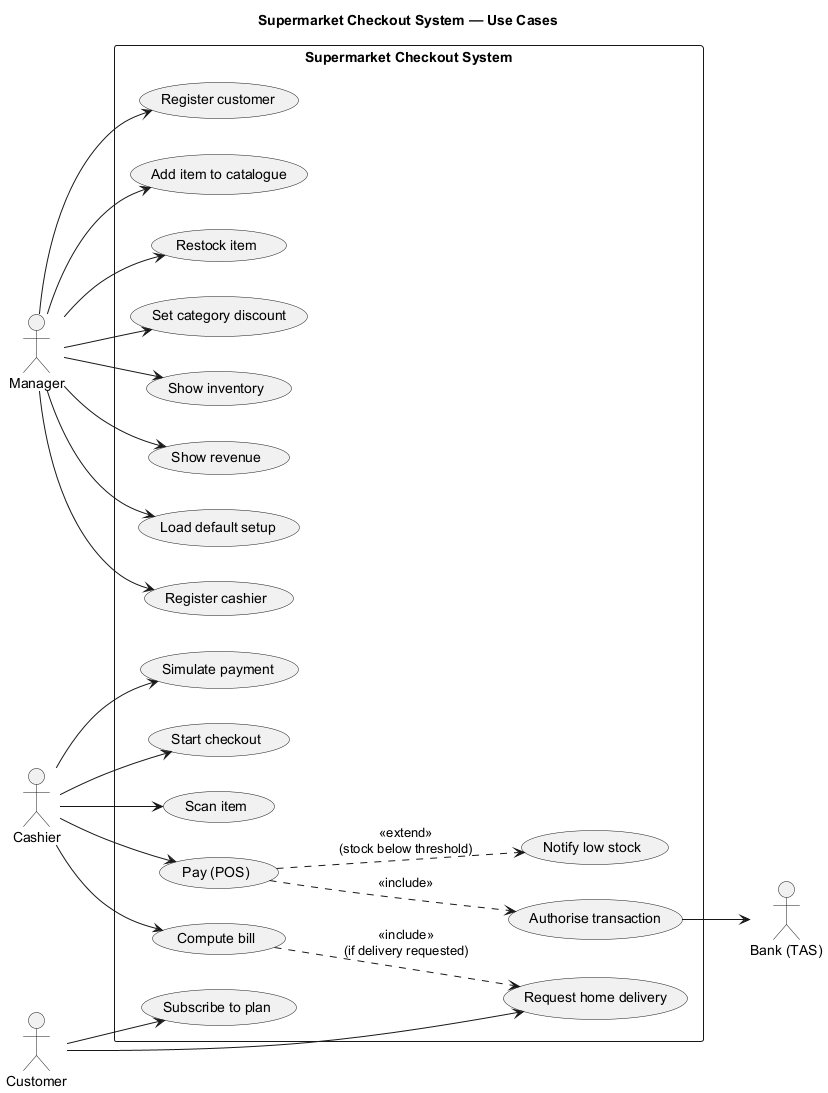
\includegraphics[width=0.8\linewidth]{use-case-diagram.png}
    \caption{Use cases for the Manager, Cashier, Customer and the Bank (TAS).}
    \label{fig:use-case}
\end{figure}

\section{Sequence Diagrams}
\label{sec:sequence}
\textit{[Commentary to be written.]}

\begin{figure}[H]
    \centering
    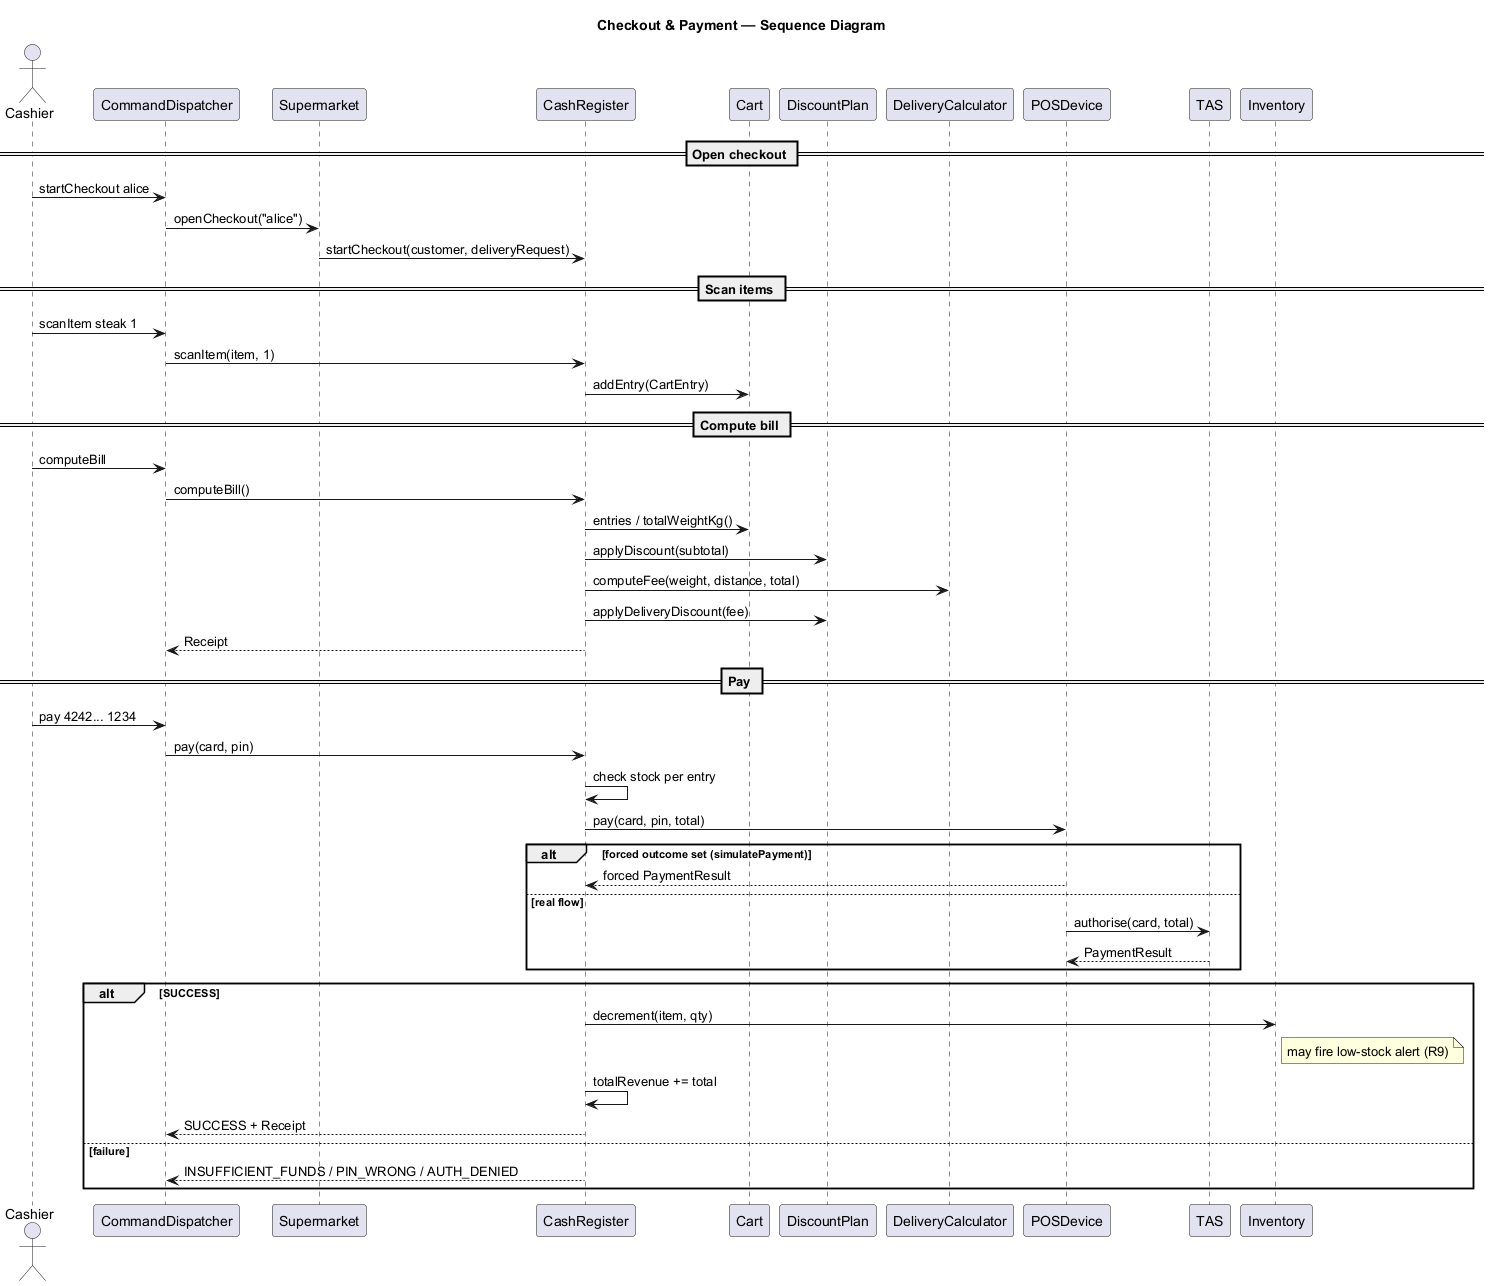
\includegraphics[width=\linewidth]{sequence-checkout-payment.png}
    \caption{Checkout and payment flow, including the forced/real payment branch
    and the post-success inventory decrement.}
    \label{fig:seq-checkout}
\end{figure}

\begin{figure}[H]
    \centering
    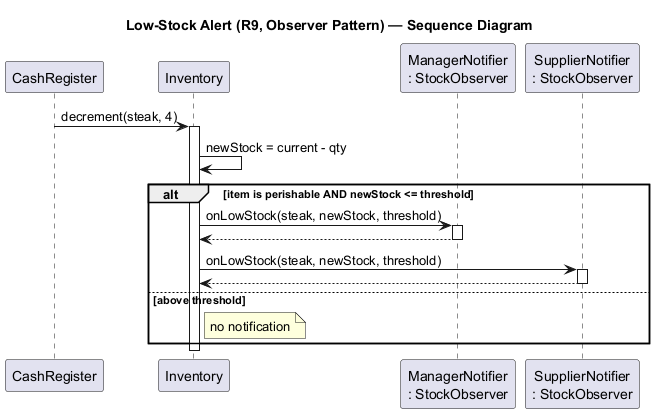
\includegraphics[width=0.65\linewidth]{sequence-low-stock-alert.png}
    \caption{Low-stock alert via the Observer pattern (R9).}
    \label{fig:seq-lowstock}
\end{figure}

\chapter{Testing}
\label{ch:testing}

Testing is a mandatory part of the project and was treated as a first-class
concern: the system is validated both by unit tests, written one class at a time,
and by end-to-end scenarios executed through the CLUI.

\section{JUnit Test Strategy}
The suite follows the instruction to provide tests for the most significant
methods of each class, excluding trivial getters and setters. It is organised as
one test class per unit, mirroring the source packages: bill computation
(\code{BillComputationTest}), the payment flow and the bank authorisation
(\code{PaymentFlowTest}, \code{TransactionAuthorisationSystemTest}), the
inventory and its Observer (\code{InventoryObserverTest}), the delivery charging
and logistics (\code{DeliveryCalculatorTest}, \code{DeliveryManagerTest},
\code{TimeSlotTest}), the discount plans and pricing policies
(\code{DiscountPlanTest}, \code{PricingPolicyTest}), and the system core and CLUI
(\code{SupermarketTest}, \code{CliDispatcherTest}). The specified system is
covered by 61 tests in the \code{v1.0} version (76 in the final version, which
adds the extension tests). The CLUI dispatcher writes to an injectable stream, so
the entire command interface is tested without any real console.

\section{Test Scenarios}
A scenario file is a list of CLUI commands run with \code{runTest}; comment lines
beginning with \code{\#} are ignored. The mandatory \code{testScenario1.txt}
reproduces a complete purchase; two further scenarios exercise the remaining
specified features. Crucially, the JUnit \code{CliDispatcherTest} executes the
very same scenario files, so the figures quoted here are checked automatically.

\begin{table}[H]
\centering
\small
\begin{tabularx}{\linewidth}{p{3cm} Y}
\toprule
\textbf{Scenario} & \textbf{What it tests} \\
\midrule
\code{testScenario1.txt} & Core happy path: a $-10\%$ category discount, a prime
subscription (\euro{}50 fee), a mixed-category checkout, the prime-halved delivery
fee (\euro{}7.50), a failed (\code{INSUFFICIENT\_FUNDS}) then successful payment,
and a low-stock alert when steak reaches~0. Final revenue \euro{}120.74. \\
\code{testScenario2.txt} & Platinum plan ($-30\%$, free delivery, \euro{}200 fee),
a dairy discount, the \code{PIN\_WRONG} and \code{AUTH\_DENIED} payment paths, a
low-stock alert cleared by \code{restock}, and a delivery refusal above 50\,kg.
Final revenue \euro{}254.236. \\
\code{testScenario3.txt} & Quantity-based bulk pricing (R3) and the smart
logistics (R10): slot booking with anti-overbooking and dynamic pricing
(peak \euro{}22.50, eco \euro{}12.00). Final revenue \euro{}15.00. \\
\bottomrule
\end{tabularx}
\caption{Test scenarios for the specified system. The extensions are exercised by
a fourth scenario described in Part~\ref{part:extensions}.}
\label{tab:scenarios}
\end{table}

\section{How to Reproduce the Tests}
The whole suite runs with a single command, and each scenario can be replayed
inside the CLUI:
\begin{lstlisting}[language=bash]
mvn test                 # compile and run every JUnit test
mvn exec:java -Dexec.mainClass="supermarket.cli.CLI"
> runTest testScenario1.txt
\end{lstlisting}
Because the scenario files are read from the project root, the automated tests
and the interactive \code{runTest} execute the same command sequences, which
makes every reported result reproducible.


\part{Extensions Beyond the Specification}
\label{part:extensions}
% Optional features added on top of the specified baseline (tagged v1.0).
\chapter{Extensions Beyond the Specification}
\label{ch:extensions}

\textit{[Skeleton --- to be written.] Built on the specified baseline (tagged
\code{v1.0}); all extensions default to no-op so the required behaviour is
unchanged. The two runnable versions of the project (specified-only and final)
are described in the README and Appendix~\ref{app:build}.}

\begin{figure}[H]
    \centering
    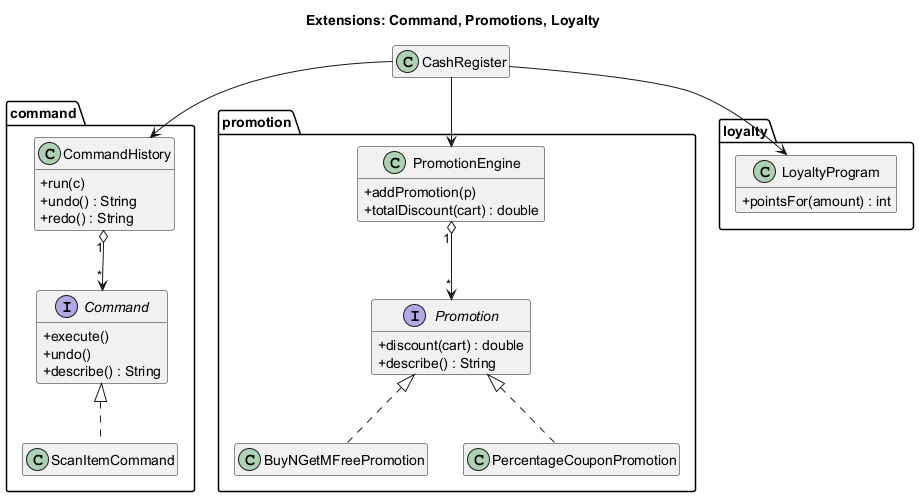
\includegraphics[width=\linewidth]{class-extensions.png}
    \caption{Class diagram of the extensions: Command (undo/redo), Promotions
    (Strategy) and Loyalty, plugged into \code{CashRegister}.}
    \label{fig:class-extensions}
\end{figure}

\section{Undo/Redo (Command Pattern)}
\textit{Reversible scan commands with a command history.}

\section{Promotions Engine (Strategy)}
\textit{Buy-N-get-M offers and percentage coupons aggregated for the bill.}

\section{Per-Category VAT}
\textit{Tax rate on each category, applied to net line prices.}

\section{Loyalty Points}
\textit{Points earned per euro spent on payment.}

\section{JavaFX Graphical Interface}
\textit{A second presentation layer over the same domain core, with a live
low-stock highlight fed by a new \code{StockObserver}. Insert a screenshot here.}


\chapter{Design Analysis and Conclusion}
\label{ch:conclusion}

\textit{[Skeleton --- to be written.]}

\section{Advantages of the Solution}
\textit{Extensibility (Open/Closed), separation of concerns, reproducible
output, two independent UIs over one core.}

\section{Limitations and Future Work}
\textit{Distance stub, slots not bound to a checkout, in-memory state; possible
next steps (persistence, REST API, point redemption).}

\section{Workload Split}
This is an individual project; all design, code, UML and tests were produced by
the single author.

\begin{table}[H]
\centering
\begin{tabularx}{\linewidth}{Y c c c c}
\toprule
\textbf{Module / Task} & \textbf{Design} & \textbf{Code} & \textbf{UML} & \textbf{Tests} \\
\midrule
\textit{All modules (placeholder list)} & \checkmark & \checkmark & \checkmark & \checkmark \\
\bottomrule
\end{tabularx}
\caption{Workload split (Enzo Jardim Vendramin).}
\label{tab:workload}
\end{table}

\section{Conclusion}
\textit{Closing paragraph on how the project meets the requirements and what the
design demonstrates.}


%---------------- APPENDICES ----------------
\appendix
\chapter{How to Build and Run}
\label{app:build}

\textit{[Skeleton.] Requires JDK 17+ (developed on JDK 21) and Maven 3.9+.}

\begin{lstlisting}[language=bash, caption={Build, test and run commands.}, label={lst:run}]
mvn test            # compile + run all JUnit tests
mvn exec:java -Dexec.mainClass="supermarket.cli.CLI"   # launch the CLUI
mvn javafx:run      # launch the JavaFX desktop GUI
\end{lstlisting}

\chapter{Complete Class Diagram}
\label{app:fullclass}

For completeness, the full class diagram of the whole system (specified core and
extensions) is reproduced below in landscape. The per-package views in
Chapter~\ref{ch:uml} are the legible decomposition of this diagram.

\begin{landscape}
\begin{figure}[H]
    \centering
    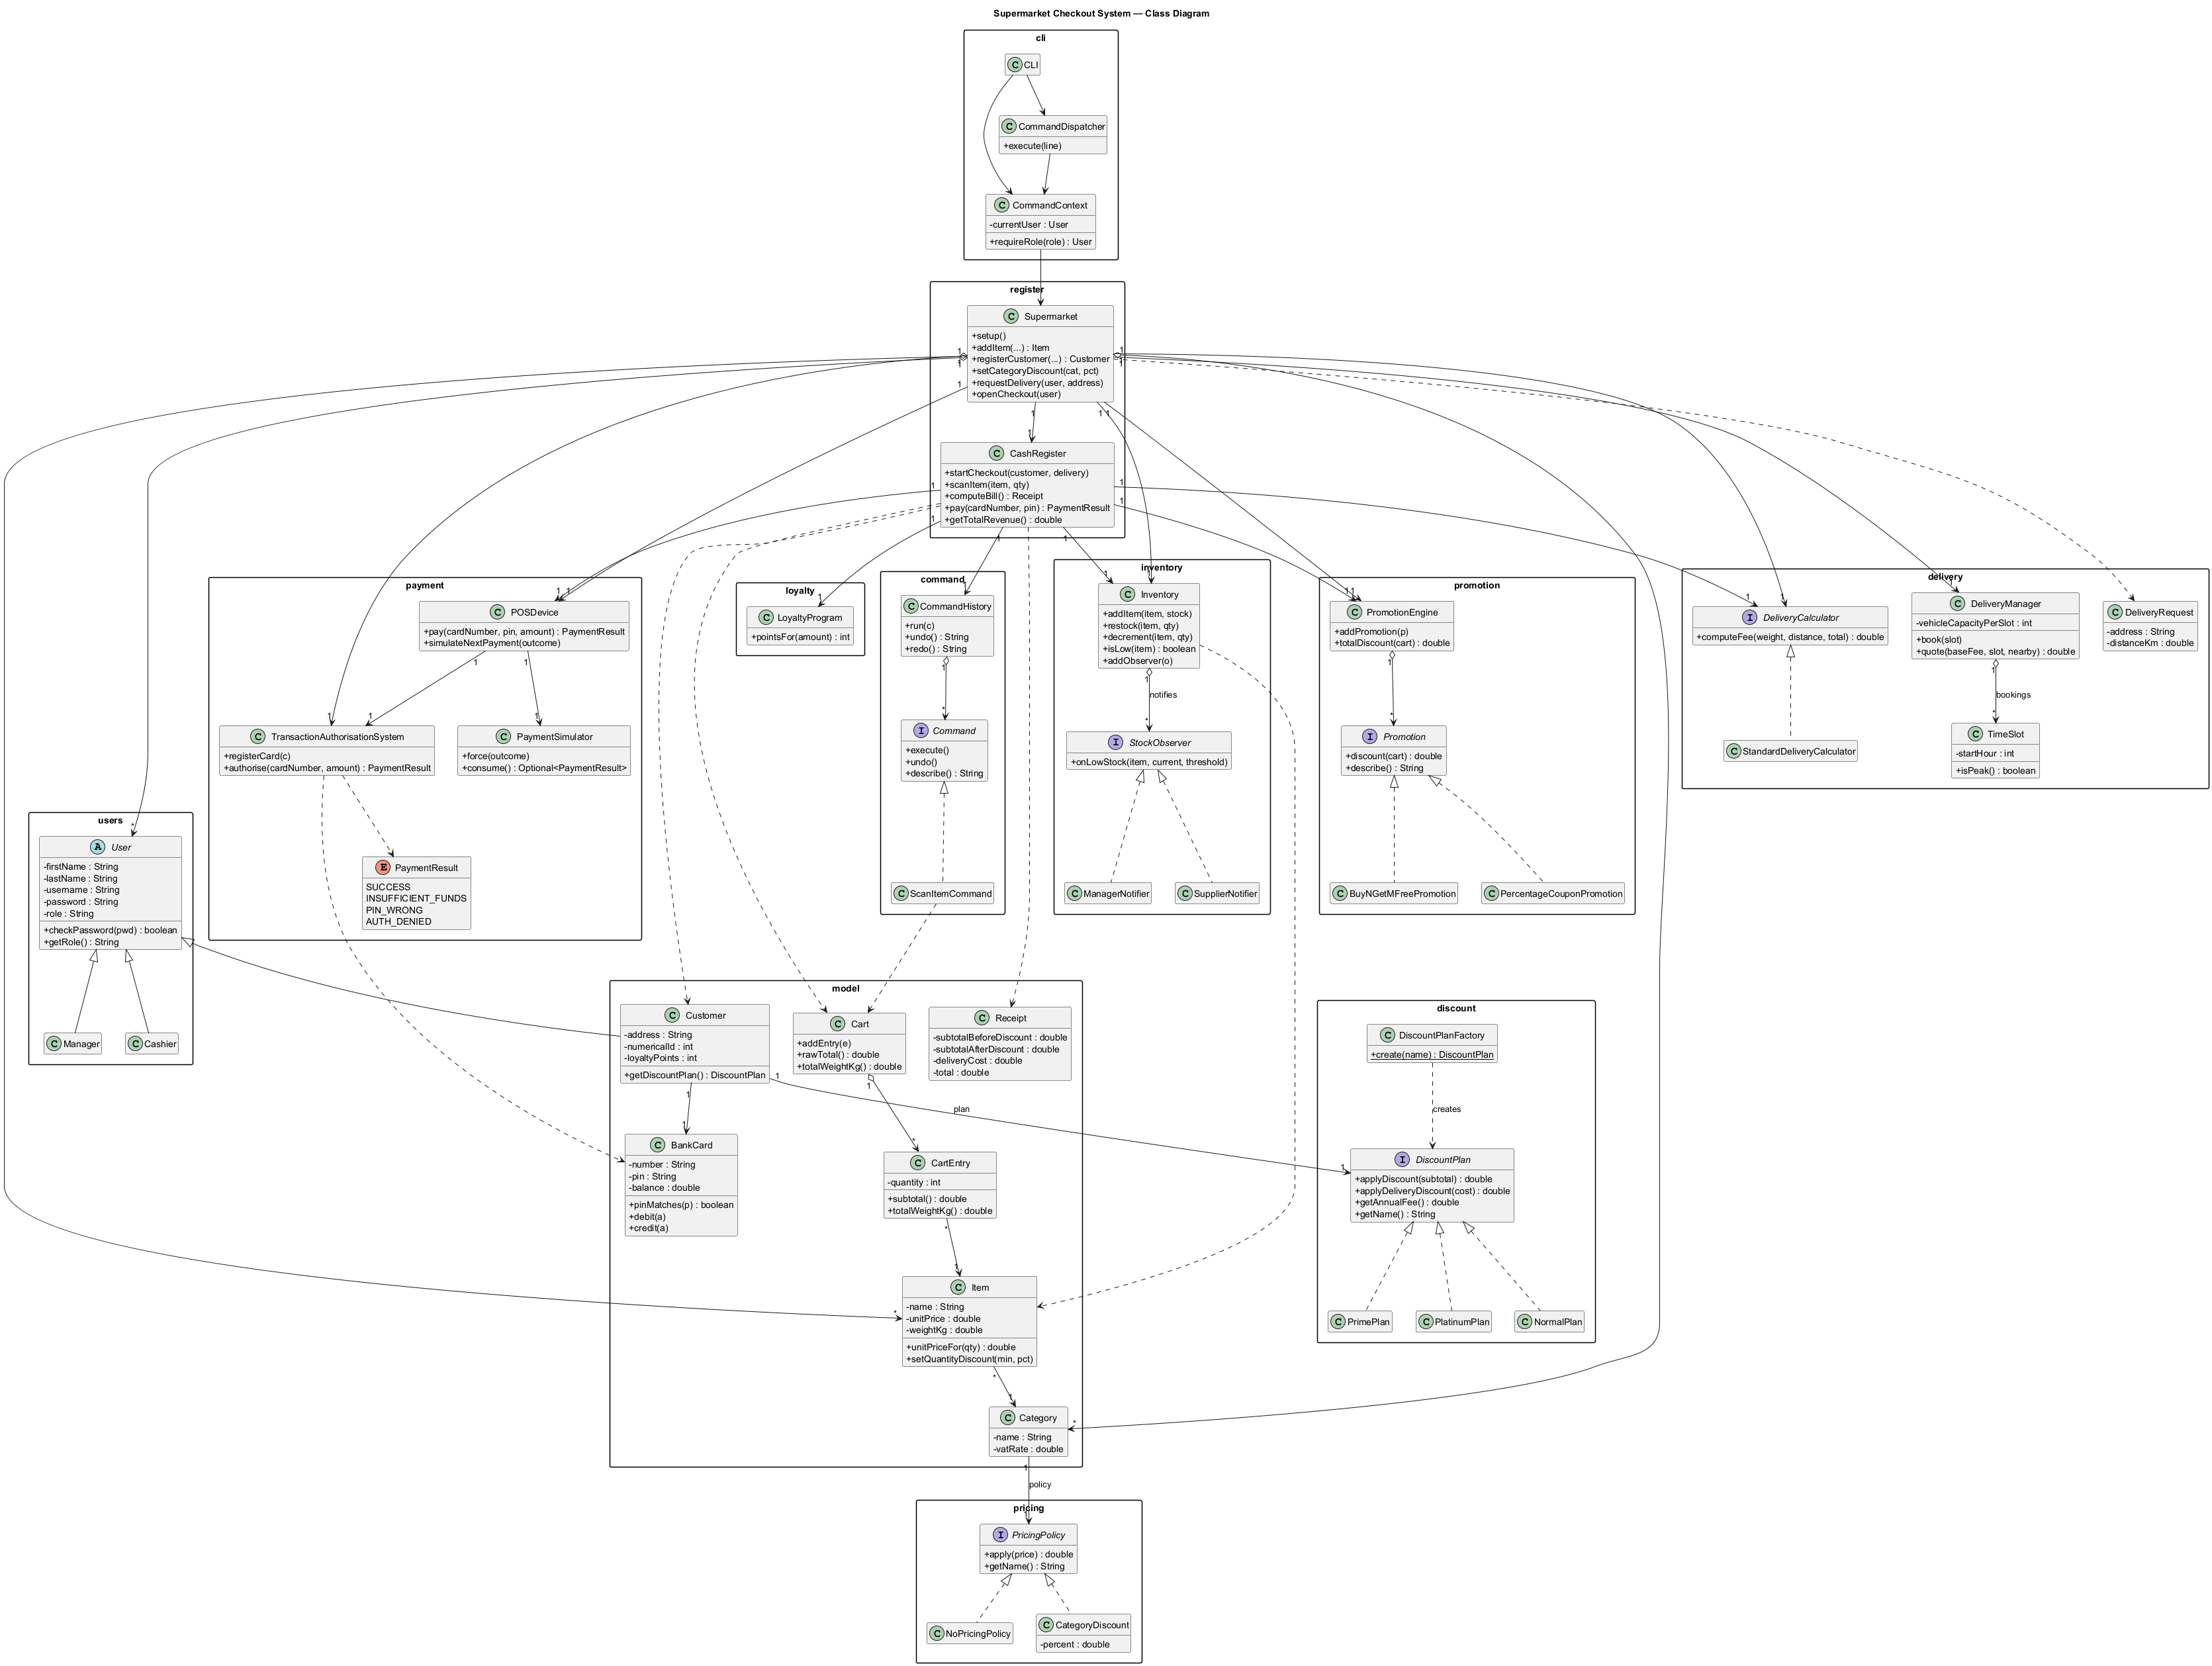
\includegraphics[height=0.92\textheight]{class-diagram.png}
    \caption{Complete class diagram (all packages).}
    \label{fig:fullclass}
\end{figure}
\end{landscape}

\chapter{Selected Code Listings}
\label{app:code}

\textit{[Skeleton] Representative excerpts will be included here, e.g. the
discount-plan Strategy interface.}

\begin{lstlisting}[language=Java, caption={The \code{DiscountPlan} strategy interface.}, label={lst:plan}]
public interface DiscountPlan {
    double applyDiscount(double subtotal);
    double applyDeliveryDiscount(double deliveryCost);
    double getAnnualFee();
    String getName();
}
\end{lstlisting}


\end{document}
